\documentclass[compress]{beamer}
\usecolortheme{default}

\usepackage{lmodern, epstopdf, multirow, array, setspace, bbm, tcolorbox, pbox, bm, mathtools, tikz}
\usepackage[T1]{fontenc}

\setbeamertemplate{frametitle}[default][center]
\setbeamertemplate{footline}{\hfill \insertframenumber/\inserttotalframenumber\hspace*{5pt}\vspace{5pt}}
\setbeamertemplate{navigation symbols}{}

\newlength{\wideitemsep}
\setlength{\wideitemsep}{\itemsep}
\addtolength{\wideitemsep}{4pt}
\let\olditem\item
\renewcommand{\item}{\setlength{\itemsep}{\wideitemsep}\olditem}
\setlength{\leftmargini}{12pt}
\setlength{\leftmarginii}{14pt}
\setbeamertemplate{itemize/enumerate subbody begin}{\vspace{6pt}}
\setbeamertemplate{itemize item}[circle]
\setbeamertemplate{enumerate item}[circle]
\setbeamertemplate{enumerate subitem}[default]

\setbeamercolor{alerted text}{fg=blue}
\setbeamersize{text margin left=1.5em,text margin right=1.5em}

\tcbset{
    colback=white,
    colframe=black,
    coltext=black,
    coltitle=blue,
    colbacktitle=white,
    boxrule=1pt,
    titlerule=0pt,
    toptitle=4pt,
    top=2pt
}

\newenvironment{changemargin}[2]{% 
  \begin{list}{}{% 
    \setlength{\topsep}{0pt}% 
    \setlength{\leftmargin}{#1}% 
    \setlength{\rightmargin}{#2}% 
    \setlength{\listparindent}{\parindent}% 
    \setlength{\itemindent}{\parindent}% 
    \setlength{\parsep}{\parskip}% 
  }% 
  \item[]}{\end{list}}
  
\newenvironment{defn}{%
  \begin{tcolorbox}[title={Definition}]%
  }{\end{tcolorbox}}
  
\newenvironment{prop}[1]{%
  \begin{tcolorbox}[title={Proposition #1}]%
  }{\end{tcolorbox}}
  
\newcommand{\cit}[1]{{\footnotesize \textcolor[rgb]{0.5,0,0}{#1}}}

% Font size for code listings (verbatim blocks); reset with \normalsize
\newcommand{\codesize}{\fontsize{7}{8.5}\selectfont}

\newcommand{\slidesetup}[1]{%
  \title{#1}%
  \subtitle{\texorpdfstring{\vspace{0.3\baselineskip}}{} {\small This version: \today}}%
  \author[Mikkel Plagborg-Moller]{ECMA 31150, Spring 2026 \texorpdfstring{\\[0.5ex]}{} University of Chicago \texorpdfstring{\\[0.5ex]}{} Department of Economics \texorpdfstring{\\[4ex]}{} Mikkel Plagborg-Moller}%
  \date{}%
}

% \circleoverlay[options]{text}
% Draws a red circle with a text box nearby on a tikz overlay.
% Options (with defaults):
%   cx=0cm, cy=0cm      - circle center (shift from page center)
%   r=1cm               - circle radius
%   tx=0cm, ty=0cm      - text box offset from circle center
%   text anchor=east    - anchor of text node (east = text left, west = text right)
%   font=\normalsize    - font size for text
\pgfkeys{
  /circleoverlay/.cd,
  cx/.store in=\cocx, cx=0cm,
  cy/.store in=\cocy, cy=0cm,
  r/.store in=\cor, r=1cm,
  tx/.store in=\cotx, tx=0cm,
  ty/.store in=\coty, ty=0cm,
  text anchor/.store in=\cotextanchor, text anchor=east,
  font/.store in=\cofont, font=\normalsize,
}
\newcommand{\circleoverlay}[2][]{%
  \pgfkeys{/circleoverlay/.cd, cx=0cm, cy=0cm, r=1cm, tx=0cm, ty=0cm, text anchor=east, font=\normalsize, #1}%
  \pgfmathsetlengthmacro{\circlediameter}{2*\cor}%
  \node[draw=red, line width=2pt, circle, minimum size=\circlediameter, inner sep=0pt]
    (tmpcirc) at ([xshift=\cocx,yshift=\cocy]current page.center) {};%
  \node[anchor=\cotextanchor, fill=white, draw=red, text=red, inner sep=4pt, align=left, font=\cofont]
    at ([xshift=\cotx,yshift=\coty]tmpcirc.center) {#2};%
}

\DeclareMathOperator*{\argmax}{argmax}
\DeclareMathOperator*{\argmin}{argmin}
\DeclareMathOperator{\diag}{diag}
\DeclareMathOperator{\var}{Var}
\DeclareMathOperator{\cov}{Cov}
\DeclareMathOperator{\corr}{Corr}
\DeclareMathOperator{\lrv}{LRV}


\slidesetup{Bayesian estimation II}

\begin{document}
\frame{
\maketitle
}

\frame{
\frametitle{Plan for this slide deck}
\begin{enumerate}
\item Bayesian forecasting
\item Modeling time-varying volatility
\item Bayesian VAR
\item Dealing with Covid-era data
\end{enumerate}
}

\frame{
\frametitle{Bayesian forecasting}
\begin{itemize}
\item Recall the Bayesian AR($p$) model from the previous slide deck.
\[y_t = c + a_1y_{t-1} + \dots + a_p y_{t-p} + u_t,\quad u_t \overset{iid}{\sim} N(0,\sigma^2).\]
\item We've seen how to generate draws from the posterior $f(\bm{\theta} \mid \bm{Y})$ of the parameters $\bm{\theta} \equiv (c,a_1,\dots,a_p,\sigma)'$ given data $\bm{Y} \equiv (y_1,y_2,\dots,y_T)'$.
\item How can we forecast $y_{T+1}$?
\item More specifically, we want to characterize the one-step-ahead \textbf{predictive distribution} of $y_{T+1}$ given $\bm{Y}$.
\end{itemize}
}

\frame{
\frametitle{Bayesian forecasting (cont.)}
\begin{itemize}
\item Density of predictive distribution:
\[f(y_{T+1} \mid \bm{Y}) = \int f(y_{T+1} \mid \bm{Y},\bm{\theta})f(\bm{\theta} \mid \bm{Y})\,d\bm{\theta}.\]
\item Algorithm for simulating from the predictive distribution: for \emph{each} posterior draw of $\bm{\theta}$, generate a draw $y_{T+1}$ from
\[(y_{T+1} \mid \bm{Y},\bm{\theta}) \sim N(c + a_1 y_T + \dots + a_p y_{T-p+1}, \sigma^2).\]
\item We can plot a histogram of the resulting draws $\lbrace y_{T+1} \rbrace$ to visualize the predictive distribution.
\item The average draw approximates $E[y_{T+1} \mid \bm{Y}]$. Could also report percentiles to get a forecast interval.
\item By design, the predictive distribution takes into account posterior uncertainty about the parameters $\bm{\theta}$.
\end{itemize}
}

\begin{frame}[fragile]
\scriptsize
\begin{verbatim}
# Extract parameter draws
draws = fit.draws_pd()
c_draws = draws['c'].values
a_draws = draws[[f'a[{l}]' for l in range(1, p+1)]].values
sigma_draws = draws['sigma'].values

# Simulate y_{T+1}
rng = np.random.default_rng(seed=31150)
x_new = y_full[-p:][::-1]  # p most recent observations in reverse order
mean_draws = c_draws + a_draws @ x_new # y_{T+1|T}
y_Tp1 = rng.normal(mean_draws, sigma_draws)
\end{verbatim}
\end{frame}

\frame{
\begin{figure}
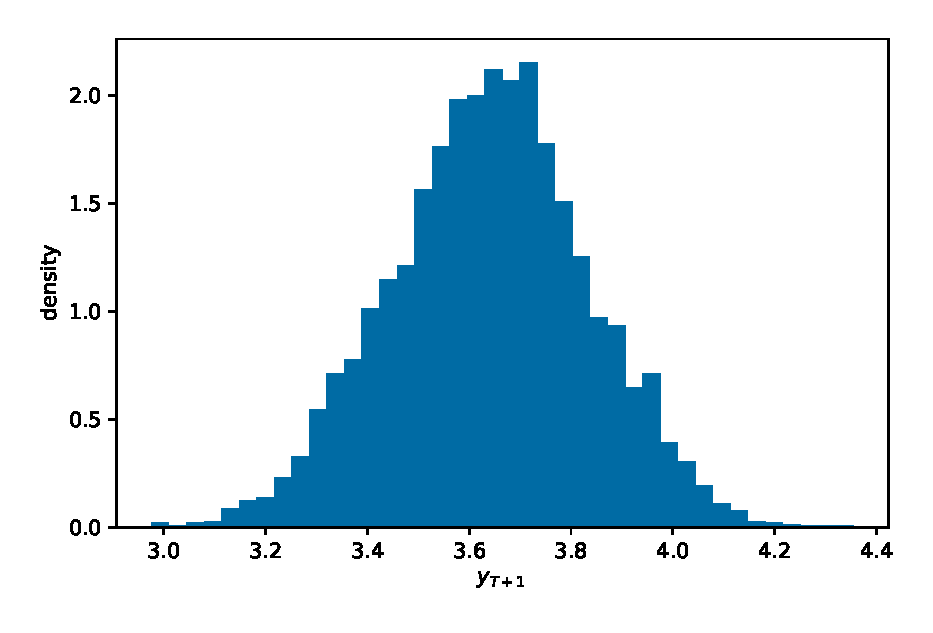
\includegraphics[width=\linewidth]{fig/bayes_ar_forecast.eps}
\end{figure}
}

\frame{
\frametitle{Time-varying volatility}
\begin{itemize}
\item So far our Bayesian model has assumed i.i.d.\ shocks $u_t$. But many time series are likely heteroskedastic.
\item \textbf{Autoregressive conditional heteroskedasticity} (ARCH) model:
\[(u_t \mid y_{t-1},y_{t-2},\dots) \sim N(0,\sigma_t^2),\]
\[\text{where}\quad \sigma_t^2 \equiv \omega + \gamma u_{t-1}^2.\]
\vspace{-\baselineskip}
\begin{itemize}
\item $\lbrace u_t \rbrace$ is a martingale difference sequence. Under stationarity, we have $E[\sigma_t^2] = \omega/(1-\gamma)$ (\alert{exercise:} verify).
\end{itemize}
\item The AR($p$) model with ARCH shocks (realistically) implies\dots
\begin{enumerate}
\item \textbf{Volatility clustering:} when $u_{t-1}^2$ is large, $u_t^2$ is also likely large.
\item $y_t$ is harder to forecast in some periods than others:
\[\var(y_t \mid y_{t-1},y_{t-2},\dots) = \sigma_t^2 \neq \text{constant}.\]
\end{enumerate}
\end{itemize}
}

\frame{
\frametitle{Time-varying volatility: likelihood}
\[(u_t \mid y_{t-1},y_{t-2},\dots) \sim N(0,\sigma_t^2), \quad \sigma_t^2 = \omega + \gamma u_{t-1}^2\]
\begin{itemize}
\item Include $\omega$ and $\gamma$ in parameter vector $\bm{\theta}$.
\item Likelihood function:
\[f(\bm{Y} \mid \bm{\theta}) = \underbrace{f(y_1,\dots,y_p \mid \bm{\theta})}_\text{ignore} \prod_{t=p+1}^T \frac{1}{\sqrt{2\pi \alert{\sigma_t^2}}}e^{-(y_t - c - \bm{x}_t'\bm{\beta})^2/(2\alert{\sigma_t^2})},\]
where
\[\alert{\sigma_t^2} = \omega + \gamma (\underbrace{y_{t-1}-c - \bm{x}_{t-1}'\bm{\beta}}_{=u_{t-1}})^2.\]
\end{itemize}
}

\begin{frame}[fragile]
Stan model file:
\bigskip
\scriptsize
\begin{verbatim}
data {
  int<lower=1> T;              // effective sample size
  int<lower=1> p;              // lag order
  vector[T] y;                 // observed series
  matrix[T, p] X;              // lag matrix
  real<lower=0> lambda;        // Minnesota prior tightness
  real<lower=0> scale_c;       // prior scale for AR intercept
  real<lower=0> scale_omega;   // prior scale for ARCH intercept
}

parameters {
  real c;                      // AR intercept
  vector[p] a;                 // AR coefficients
  real<lower=0> omega;         // ARCH intercept
  real<lower=0,upper=1> gamma; // ARCH parameter
}
\end{verbatim}
\normalsize
(continued on next slide)
\end{frame}

\begin{frame}[fragile]
\codesize
\begin{verbatim}
transformed parameters {
  vector[T] sigma2;            // conditional variances
  {
    vector[T] u = y - (c + X * a);
    sigma2[1] = omega / (1 - gamma); // initialize at unconditional mean
    for (t in 2:T)
      sigma2[t] = omega + gamma * square(u[t-1]);
  }
}

model {
  // Minnesota prior on AR coefficients
  for (l in 1:p) {
    real m_ = (l == 1) ? 1.0 : 0.0;
    real sd_ = lambda / l;
    a[l] ~ normal(m_, sd_);
  }

  // Intercept and ARCH priors
  c ~ normal(0, scale_c);
  omega ~ normal(0, scale_omega);
  gamma ~ beta(1.1, 1.1); // nearly uniform on [0,1]

  // Likelihood (vectorized)
  y ~ normal(c + X * a, sqrt(sigma2));
}
\end{verbatim}
\end{frame}

\frame{
\begin{figure}
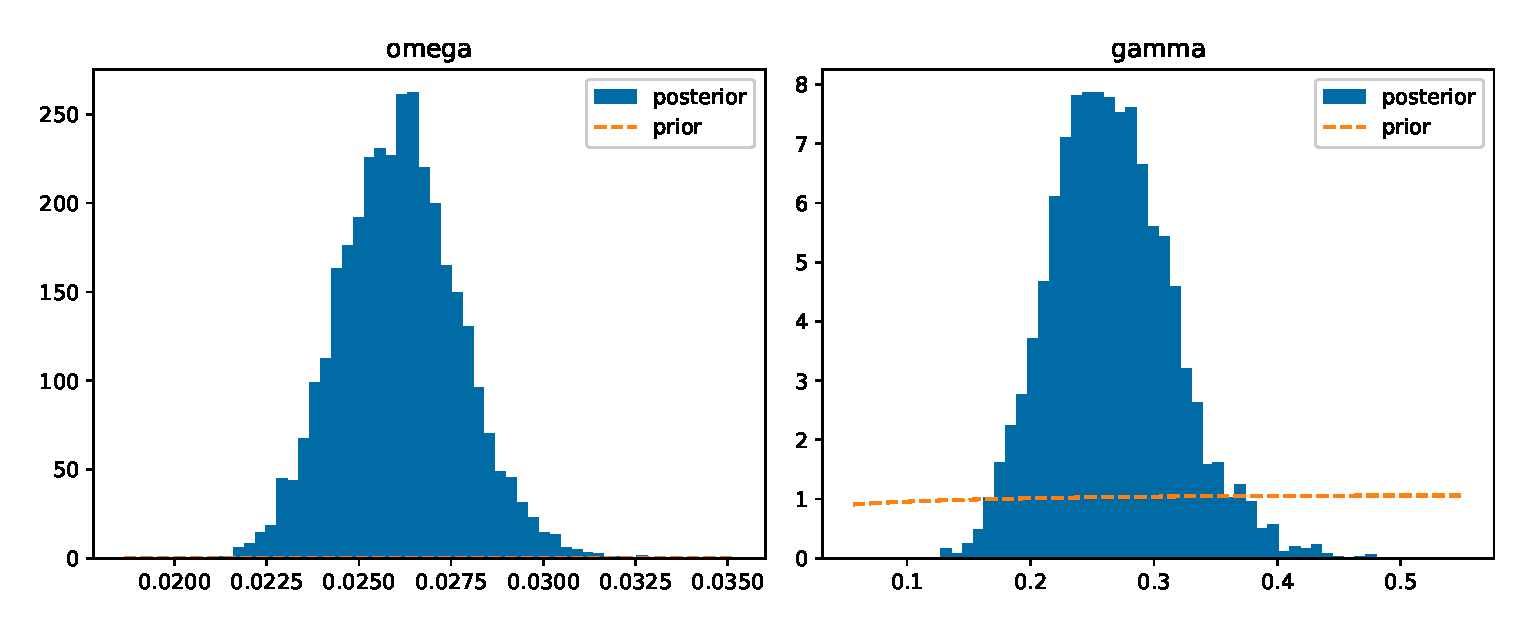
\includegraphics[width=\linewidth]{fig/bayes_arch_posterior.eps} \\
\bigskip
Note: prior on $\omega$ is so diffuse that it's barely visible.
\end{figure}
}

\frame{
\begin{figure}
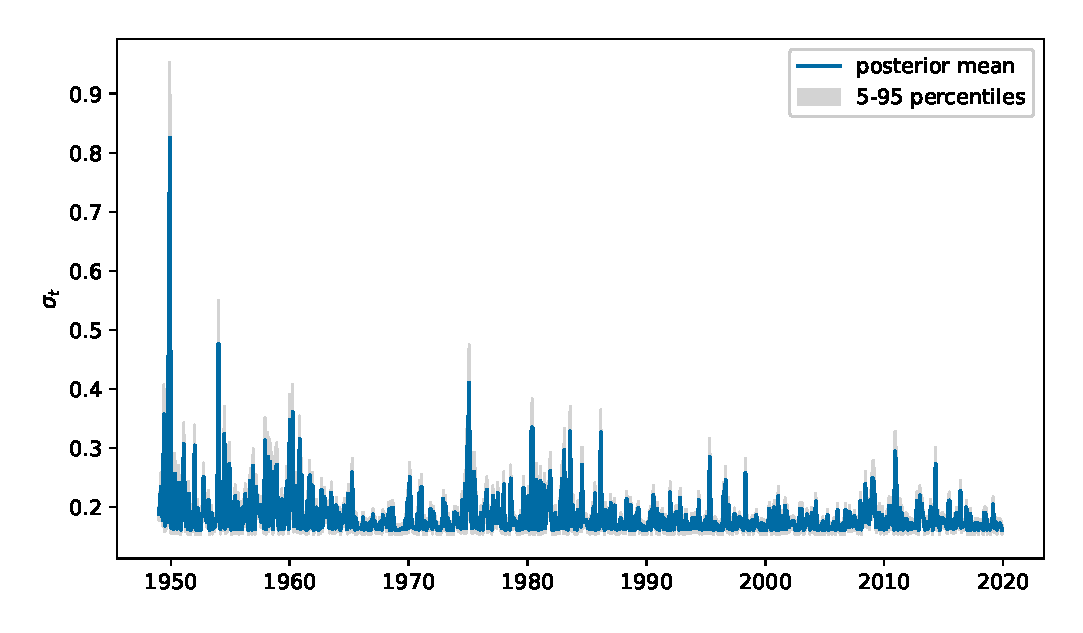
\includegraphics[width=\linewidth]{fig/bayes_arch_volatility.eps} \\
\bigskip
Posterior distribution of $\lbrace \sigma_t \rbrace_{t=p+1}^T$ -- notice volatility clustering
\end{figure}
}

\frame{
\begin{figure}
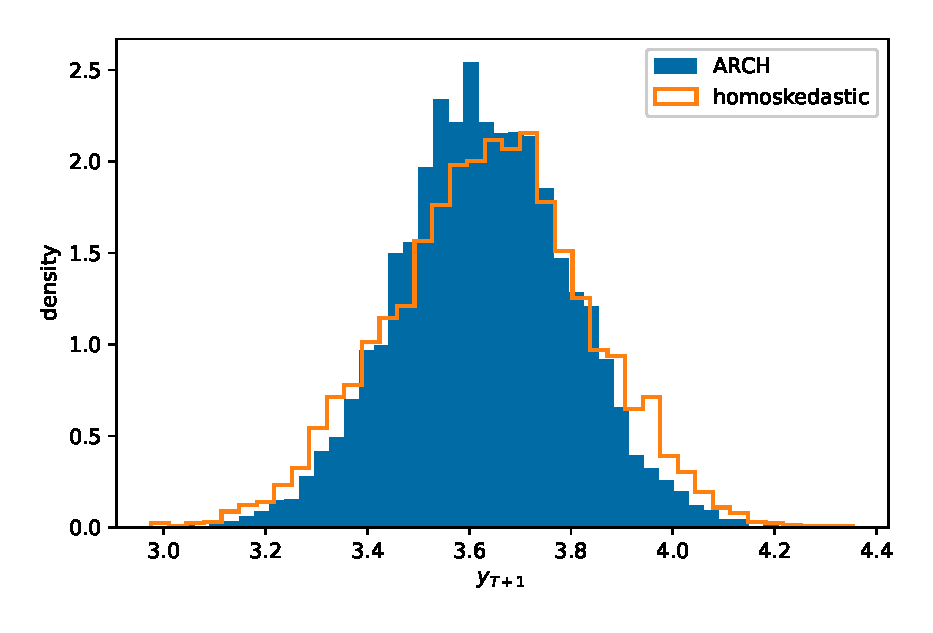
\includegraphics[width=\linewidth]{fig/bayes_arch_forecast.eps} \\
One-step-ahead predictive distribution: ARCH vs.\ homoskedastic shocks
\end{figure}
}

\frame{
\frametitle{Time-varying volatility: GARCH}
\begin{itemize}
\item \textbf{Generalized ARCH} (GARCH) model:
\[(u_t \mid y_{t-1},y_{t-2},\dots) \sim N(0,\sigma_t^2),\]
\[\sigma_t^2 = \omega + \gamma u_{t-1}^2 + \delta \sigma_{t-1}^2.\]
\item Could include more lags of $u_t^2$ and/or $\sigma_t^2$ on the right-hand side.
\item You'll be working with this model on the problem set.
\end{itemize}
}

\frame{
\frametitle{Bayesian VAR (BVAR)}
\begin{itemize}
\item VAR($p$) model (homoskedastic for simplicity):
\[\bm{y}_t = \bm{c} + \bm{A}_1 \bm{y}_{t-1} + \dots + \bm{A}_p \bm{y}_{t-p} + \bm{u}_t,\quad \bm{u}_t \overset{iid}{\sim} N(\bm{0},\bm{\Sigma}).\]
\item Data: $\bm{Y} \equiv (\bm{y}_1,\dots,\bm{y}_T)'$, dimension $T \times n$.
\item Parameters: $\bm{\theta} = \lbrace \bm{c},\bm{A}_1,\dots,\bm{A}_p,\bm{\Sigma} \rbrace$.
\end{itemize}
}

\frame{
\frametitle{BVAR: Minnesota prior}
\begin{itemize}
\item $A_{\ell,ij}$: $(i,j)$ element of $\bm{A}_\ell$.
\item Prior means:
\[E[A_{\ell,ij}] = \begin{cases}
1 & \text{if } i=j \text{ and } \ell=1, \\
0 & \text{otherwise}.
\end{cases}\]
\item Each variable $y_{it}$ is shrunk towards a univariate random walk: $y_{it} = y_{i,t-1} + u_{it}$.
\item Prior belief: limited Granger causality from one variable to another.
\end{itemize}
}

\frame{
\frametitle{BVAR: Minnesota prior (cont.)}
\begin{itemize}
\item Prior variances:
\[\var(A_{\ell,ij}) = \begin{cases}
\left(\frac{\lambda}{\ell}\right)^2 & \text{if } i=j, \\
\left(\frac{\lambda \kappa}{\ell} \times \frac{\hat{\sigma}_i}{\hat{\sigma}_j}\right)^2 & \text{otherwise}.
\end{cases}\]
\item $\lambda$ controls overall prior variance.
\item $\kappa$ controls relative variance on \emph{cross-variable} coefficients ($i \neq j$).
\begin{itemize}
\item Typical values in literature: $\lambda=0.2$, $\kappa=0.3$.
\end{itemize}
\item Lower variance (more dogmatic beliefs) on longer lags $\ell$.
\item $\hat{\sigma}_i$: estimate of $\sqrt{\var(u_{it})}$ (e.g., from preliminary OLS VAR).
\item Scaling $\hat{\sigma}_i/\hat{\sigma}_j$ adjusts for disparate units of $y_{it}$ and $y_{jt}$.
\end{itemize}
}

\frame{
\frametitle{BVAR: Minnesota prior (cont.)}
\begin{itemize}
\item Example: bivariate VAR(2), with priors in blue.
\bigskip
\begin{align*}
y_{1t} &= c_1 + \underset{\alert{N\big(1,\lambda^2\big)}}{A_{1,11}}y_{1,t-1} + \underset{\alert{N\big(0,(\lambda\kappa\frac{\hat{\sigma}_1}{\hat{\sigma}_2})^2\big)}}{A_{1,12}}y_{2,t-1} \\
&\quad + \underset{\alert{N\big(0,(\frac{\lambda}{2})^2\big)}}{A_{2,11}}y_{1,t-2} + \underset{\alert{N\big(0,(\frac{\lambda\kappa}{2}\frac{\hat{\sigma}_1}{\hat{\sigma}_2})^2\big)}}{A_{2,12}}y_{2,t-2} + u_{1t} \\[\baselineskip]
y_{2t} &= c_2 + \underset{\alert{N\big(0,(\lambda\kappa\frac{\hat{\sigma}_2}{\hat{\sigma}_1})^2\big)}}{A_{1,21}}y_{1,t-1} + \underset{\alert{N\big(1,\lambda^2\big)}}{A_{1,22}}y_{2,t-1} \\
&\quad + \underset{\alert{N\big(0,(\frac{\lambda\kappa}{2}\frac{\hat{\sigma}_2}{\hat{\sigma}_1})^2\big)}}{A_{2,21}}y_{1,t-2} + \underset{\alert{N\big(0,(\frac{\lambda}{2})^2\big)}}{A_{2,22}}y_{2,t-2} + u_{2t}
\end{align*}
\end{itemize}
}

\begin{frame}[fragile]
Excerpts from Stan model file:
\smallskip
\scriptsize
\begin{verbatim}
transformed data {
  // Build mean and stdev of Minnesota prior
  matrix[n, n*p] A_mean;
  matrix[n, n*p] A_std;
  for (l in 1:p) {      // lag
    for (i in 1:n) {    // equation
      for (j in 1:n) {  // regressor
        int col = (l - 1) * n + j;
        A_mean[i, col] = (l == 1 && i == j) ? 1 : 0;
        A_std[i, col] = (i == j)
          ? lambda / l
          : (lambda / l) * (kappa * scale_sigma[i] / scale_sigma[j]);
      }
    }
  }

  // Scale matrix for Sigma prior
  matrix[n, n] Sigma_scale = diag_matrix(square(scale_sigma));
}
\end{verbatim}
\smallskip
\normalsize
(continued on next slide)
\end{frame}

\begin{frame}[fragile]
\scriptsize
\begin{verbatim}
model {
  // Minnesota prior on VAR coefficients
  to_vector(A) ~ normal(to_vector(A_mean), to_vector(A_std));

  // Intercept prior
  c ~ normal(0, scale_c);

  // Prior on innovation var-cov matrix
  Sigma ~ inv_wishart(n + 2, Sigma_scale);

  // Likelihood
  for (t in 1:T)
    Y[t] ~ multi_normal(c + A * X[t]', Sigma);
}
\end{verbatim}
\bigskip
\normalsize
Note: the inverse-Wishart distribution is a distribution on the space of $n \times n$ variance-covariance matrices.
\end{frame}

\frame{
\frametitle{BVAR: sampling}
\begin{itemize}
\item Stan takes substantially longer to sample from this model due to the many parameters.
\item One can design much faster samplers for this specific model and prior. There is a huge literature on computational tricks for BVARs.
\item Stan, however, makes it easy to modify the model or prior (e.g., add time-varying volatility).
\end{itemize}
}

\frame{
\frametitle{Bayesian SVAR}
\begin{itemize}
\item How to use BVARs for causal inference?
\item Given the posterior draws of the VAR parameters $\bm{\theta} = \lbrace \bm{c},\bm{A}_1,\dots,\bm{A}_p,\bm{\Sigma} \rbrace$, we can compute the Cholesky-identified IRFs corresponding to each draw:
\[\bm{\Theta}_h = \begin{pmatrix} \bm{I}_{n \times n}, \bm{0}_{n \times n(p-1)} \end{pmatrix} \bm{A}^h \begin{pmatrix} \bm{H} \\ \bm{0}_{n(p-1) \times n} \end{pmatrix},\]
where $\bm{H} \equiv \text{Cholesky}(\bm{\Sigma})$, and $\bm{A}$ is the $(np) \times (np)$ companion form matrix corresponding to $\bm{A}_1,\dots,\bm{A}_p$.
\item This gives us posterior draws of the structural IRFs.
\item Similarly for FEVDs.
\end{itemize}
}

\frame{
\begin{figure}
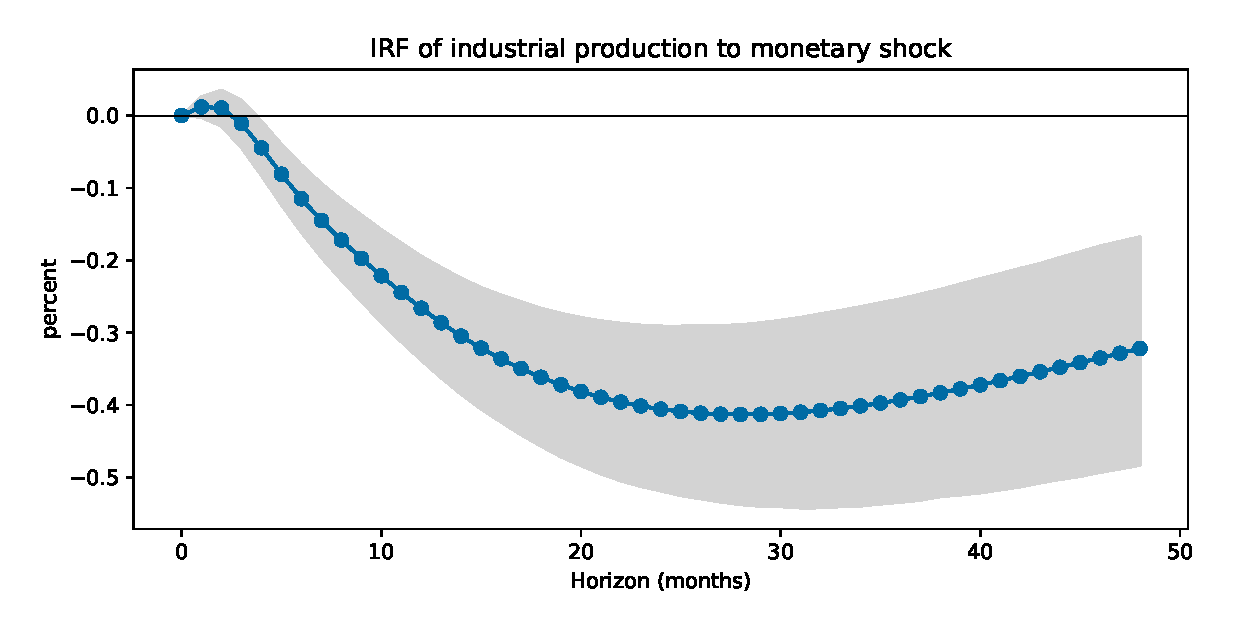
\includegraphics[width=\linewidth]{fig/bayes_svar_irf.eps} \\
\bigskip
6-variable Cholesky-identified SVAR (as in earlier slide deck)
\medskip

Blue dots: posterior means; gray band: posterior 68\% credible intervals
\end{figure}
}

\begin{frame}[fragile]
\frametitle{Hierarchical Bayes}
\begin{itemize}
\item Results may be sensitive to the \textbf{hyper-parameters} $\lambda$ and $\kappa$ in the Minnesota prior, since they determine the degree of shrinkage.
\item It would be nice to have a data-dependent way to select them.
\item \textbf{Hierarchical Bayes}: treat these as unknown parameters themselves, with their own ``hyper-priors''.
\item In Stan, just move \texttt{lambda} and \texttt{kappa} to the \texttt{parameters} block. In the \texttt{model} block, add their priors:
\smallskip
\begin{verbatim}
lambda ~ gamma(0.25, 1.25); // mean 0.2, stdev 0.4
kappa ~ gamma(0.25, 0.833); // mean 0.3, stdev 0.6
\end{verbatim}
\item Further reading: Giannone, Lenza \& Primiceri (2015).
\end{itemize}
\end{frame}

\frame{
\frametitle{Prior shrinkage and causal inference}
\begin{itemize}
\item Prior shrinkage reduces the variance of estimators, but at the expense of higher bias (unless our prior beliefs are totally accurate).
\item BVARs often outperform OLS VAR estimates when it comes to mean squared error (for forecasts or parameters).
\item However, as we discussed when comparing LP and SVAR, even a bit of bias can cause severe coverage distortions. These distortions get worse the tighter are our priors.
\item I would not recommend using BVARs with the conventional Minnesota prior for \emph{causal inference}. BVARs should only be employed with a very long lag order $p$ and much more diffuse priors than we have imposed above.
\end{itemize}
}

\frame{
\frametitle{Modeling the Covid shock}
\begin{itemize}
\item Textbook time series models have a difficult time dealing with data from March 2020 and the following few months.
\item Key economic time series showed extreme jumps/swings in these months.
\item If we estimate a model that does not explicitly model the Covid period, our estimated shock volatility parameters will be largely driven by those few hard-to-fit observations.
\begin{itemize}
\item Could mess up causal inference or post-2020 forecasts.
\end{itemize}
\end{itemize}
}

\frame{
\begin{figure}
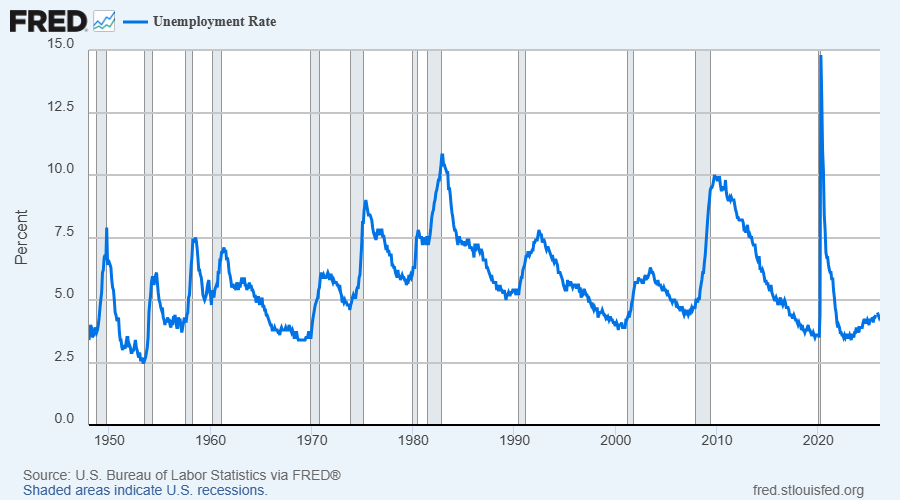
\includegraphics[width=\linewidth]{fig/fred_unrate.png}
\end{figure}
}

\frame{
\frametitle{Modeling the Covid shock (cont.)}
\begin{itemize}
\item We can allow for heightened volatility in the Covid period by letting our shock volatility parameter shift in those periods.
\item AR($p$) example:
\[y_t = c + a_1y_{t-1} + \dots + a_p y_{t-p} + u_t,\quad u_t \overset{indep}{\sim} N(0, \sigma_t^2),\]
\[\text{where}\quad \sigma_t \equiv (1+\eta s_t)\sigma, \quad s_t \equiv \begin{cases}
1 & \text{for } t \in \text{Covid}, \\
0 & \text{otherwise}.
\end{cases}\]
\item The parameter $\eta\geq 0$ captures the volatility shift.
\item Estimation in Stan only requires minor modifications of our earlier AR($p$) model file.
\item More detailed guidance: Lenza \& Primiceri (2022).
\end{itemize}
}

\frame{
\frametitle{What did we learn?}
\begin{itemize}
\item Bayesian forecasting, predictive distribution
\item ARCH, GARCH
\item BVAR
\begin{itemize}
\item Minnesota prior
\item Cholesky identification
\item Hierarchical Bayes
\end{itemize}
\item Modeling Covid as a volatility shift
\end{itemize}
}

\frame{
\frametitle{Looking ahead}
\begin{itemize}
\item State space models: very rich class of models with latent variables
\item Inferring the values of latent variables
\item Factor models
\end{itemize}
}

\end{document}
